\documentclass[a4paper,fontsize=12pt]{article}
\usepackage{fontspec}                 % loaded by polyglossia, but included here for transparency
\usepackage{polyglossia}
\usepackage{indentfirst}              % Insert "Red line"

\usepackage{graphicx}          % Insert images

\setmainlanguage{russian}
\setotherlanguage{english}

\usepackage[left=3.5cm,right=2cm,top=2.5cm,bottom=2.5cm,bindingoffset=0cm]{geometry}
% XeLaTeX can use any font installed in your system fonts folder
% Linux Libertine in the next line can be replaced with any
% OpenType or TrueType font that supports the Cyrillic script.

\newfontfamily\russianfont[Script=Cyrillic]{Arial}

\begin{document}

% \maketitle\clearpage
% \restoregeometry
% \pagenumbering{arabic}
% \tableofcontents\clearpage

%

\begin{titlepage}
  \thispagestyle{empty}

  \begin{center}
    \Large{\textbf{Национальный исследовательский университет МИЭТ}}

    \vspace{5cm}

    \huge{\textbf{\textit{Курсовая работа}}}

    \large{по дисциплине}

    \large{«Квантовая теория и статистическая физика»}

    \vspace{1cm}

    \huge{\textbf{\textit{Оценка апроксимации для эффективной топографической симуляции ионно-лучевых процессов: 10К эВ $Ar$ на $Si$}}}
  \end{center}

  \vspace{1cm}

  \begin{flushright}
    \textbf{Выполнил:}                  \linebreak
    Студент группы ЭКТ-26               \linebreak
    Чечетин П. Е.                       \linebreak
    \textbf{Проверил:}                  \linebreak
    учёная степень, учёное звание       \linebreak
    ФИО преподавателя                   \linebreak
  \end{flushright}

  \vfill

  \begin{center}
    \Large{Москва – 2013}
  \end{center}
\end{titlepage}

\newpage
\tableofcontents

\newpage
\section{Резюме}
Основное предположение о существовании эффективной топографической симулиции состоит в том что распыление - это локальный процесс который зависит только от угла столкновения и не зависит от формы поверхности. Если учитывать переосаждение, распылённые атомы переосаждаются и не вызывают дальнейшего распыления когда они сталкиваются с другим участками поверхности. Более того угловое распределение распылённых атомов определяется законом косинуса. Если учитывать ионное отражение, тогда ионы не теряют энергию в процессе обратного рассеяния. Используя симуляцию бинарных столкновений (IMSIL) и сравнивая их с результатами полученными с помощью топографического симулятора ($IonShaper^{®}$) мы видим что всем этим предположениям нужны уточнения для симуляции наноструктур прнебрегая распыление распылённых атомов. Кроме того мы показываем что не локальные модели в основном справедливы для ионно-лучевого наведённого облучения внутренней структуры.

\section{Введение}
Ионные лучи это многостароннее и всё больше используемое стредства для создания наноструктур либо c помощью прямого фрезерования либо путём процессов в газовой среде. Настоящее обучение мотивированно усилиями создать штампы для нано-литографии c массивными многоионными лазерными системами. Во всех приложениях симуляция может помочь понять физические процессы и оптимизировать форму структур.


\begin{figure}[h]
    \centering
    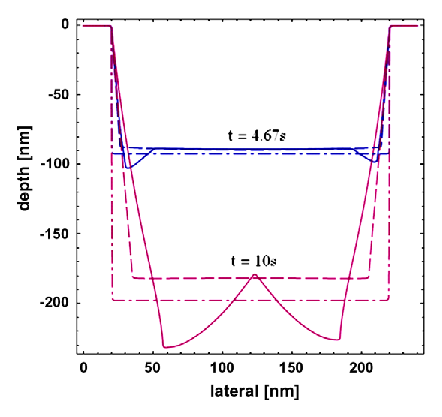
\includegraphics[width=6cm]{images/1.eps}
    \caption{This is a demo figure}
    \label{fig:demo1}
\end{figure}

Большинство сущестувующих алгоритмов для численно эффективных топографических симуляции ионно-лазерных процессов моделирует поверхность проникновения явно, в соответствии с историей, точки поверхности считались соединёнными прямыми сегментами. Все алгоритмы базируются на предположении что рассеивание - это функция угла между направлением ионов и локальной нормалью поверхности. Обычно это хорошая апрокимация для структур в диапозоне микрометров, но это становится под вопросом когда характерный размер становится меньше. Только некоторые алгоритмы включают переосаждение и только несколько распыление отраженных ионов. Эти эффекты в основном важны в структурах с большим отношением сторон как в глубоких ямах. Рисунок 1 показывает контуры ям облучённых 200 нм широко гомогенным ионным лучём в два раличных момента времени, посчитанных с помощью програмного обеспечения $IonShaper^{®}$. В любое время симуляция без переосаждения и отражения (штрих-пунктирная линии) сравнима с симуляцией учитывающей только переосаждение (пунктирная линия) и учитывающей как переосаждение так и отражение (сплошная линия). Можно заметить что переосаждение атомов рассееных из дна ямы ведёт к уменьшению ямы по направлению ко дну. На следующей стадии (не показанно), переосаждение от граней ко дну и к другой грани ведёт к уменьшению эфективности фрезерования. Отражение ионов от граней ведёт к формированию микроям на дне ямы возле граней. Более того, увеличение излучение на наклонёную поверхность микротрещин ведёт к дополнительному переосаждению на грани.

В подсчёте переосаждённого потока, закон косинуса используется чтобы описать угловое распределение распылённых ионов. Обратное рассеение предпологаеться без потери энергии. Далее, распылённые атомы которые достигают другую точку поверхности переосаждаясь там и не вызывают рассеение. Эти предположения как и локальная аппрокимация рассеения исследуются в этой статье используя симуляцию бинарных столкновений. Мы ограничиваем себя в 10к эВ $Ar$-ионы и $Si$-мишени т.к. это наш текуший фокус интересов.

\section{Симуляция}
\subsection{Топографическая симуляция}

Двухмерная(2D) топограческая симуляция выполняются с $IonShaper^{®}$ программой. Коротко, поверхность описывается достаточным кол-вом точек которые движутся перпендикулярно к среднему наклону смежных сегментов. Скорость точек считается от потока атомов распылённых ионным лучом и от ионов отражённых от других частей поверхности и от потока переосаждённых атомовов исходящих от распыления от остальных точек поверхности. Распыление считается локальным процессом, т.е. поток распылённых частиц в определённой точке пространства зависит только от потока падаюших ионов в эту точку и их угла относительной нормальни поверхности.

В действительности, из-за ограниченных пределов отскока, распылённые атомы испускаются из облости вокруг точки падения. Чтобы исследовать этот эффект мы дополнительно реализовали не локальную модель потока расплыления. Кол-во отскоков в определённой точке поверхности (точке назначения) от столкновения ионов в другой точке поверхности (источнике) расчитывается от расстояния между двух точек и угла между прямой соединяющей эти точки и направлением падающих ионов.

Изначальная версия $IonShaper^{®}$ включала модель вынужденного лучевого напыления которое включало посчёт предшествующей зоны наблюдения и простую реализацию нелокального эффекта ионов/напылении. Было показанно что доля напыления пропоруианальна кол-ву отскоков достигших поверхность. Поэтому мы улучшили модель напыления используя модель основанную на отскоках опиисанную выше.

\subsection{Бинарная симуляция столкновений}

Бинарная симуляция столкновений сделанна с IMSIL алгоритмом. IMSIL было использованно для имплантационных исследований для одна и двух мерных целей. В этой работе мы только используем аморфные цели, т.к. $Si$ просто аморфиризуется при ионом бомбондировании. IMSIL был улучшен для расчётов распыления в двух аспектах. Первое, реализована планарная модель поверхностного потенциала. Хотя это достаточно очивидно для 1D целей, это более запутанно в случае поверхнсти данной в полигонах, в случае 2D из-за необходимости отслеживать трактории на некотором расстоянии вне цели и считать нормаль поверхности там.Мы делает это путём охвата зоны симуляции прямоугольной сеткой и считаем расстояние от каждой ячейки до поверхности. В процессе симуляции траектории отскоков расстояния отскоков от поверхности считается с помощью интерполяции в табличных величинах. Если расстояние от новой точки отскока из поверхности превышает максимум параметра $p_{max}$, тогда отскок возвращается в точку предидущего свободного полёта который есть расстояние $p_{max}$ от поверхности. Нормаль поверхности в этой точке считается через градиент функции расстояния. В основном, отскоки покидающие поверхность проверяются путём помещения цели куда-нибудь ещё. В целях обучения, однако, отскоки останавливаются когда они покидают цель. Путём подгонки эксперементалього выхода распыления была определенна эффективная поверхнастная энергия связи в 4.1 эВ.

Второе, особое внимание должно быть уделенно чтобы обработать всплески столкновений правильно. Чтобы избижать нереалистично близких столкновений когда помещаем цель, ионы должны начинать с расстояния $p_{max}$ от поверхности. Только если внутри цели атомы цели настигаются тогда происходят столкновения. Однако, даже тогда результаты могут зависить от предположения о путях свободного пролёта. Это потому что распределение пути свободного пролёта неявно определяет шероховатость поверхности. Поэтому мы используем распределение Пуассона для пути свободного пробега которое обеспечивает хорошую модель цели. Вместе с игнорированием столкновений вне цели это гарантирует постоянную атомную плотность внутри и нулевую плотность вне цели.

\section{Результаты}
\subsection{Угловое распределение}

Рис.1 показывает угловое распределение распылёных и обратно рассеянных атомов полученное путём симуляции бинарных столкновений для углов наклона
  $0^{\textdegree}$,
  $40^{\textdegree}$,
  $70^{\textdegree}$,
  $87^{\textdegree}$.

C увеличением угла наклона распределение возростающее отклоняется от закона косинуса (показанно на сфере). Отклонение важно в основном при фрезерования глубоких ям т.к. поток в обратном направлении (направо Рис. 2) определяет сколько атомов могут покинуть яму.
Угловое распределение обратно рассеянных электронов может быть только грубо описанно зеркальным отражением (прямые пунктирные линии). Распределение более смещенно по направлению *exit angles perpendicular to the surface* с большым стандартным отклонением в меньших углах наклона. Угловое распределение отраженных ионов определяет поверхность микроям показанных на Рис. 1 и поэтому должно быть описано точно.

\begin{figure}[h]
    \centering
    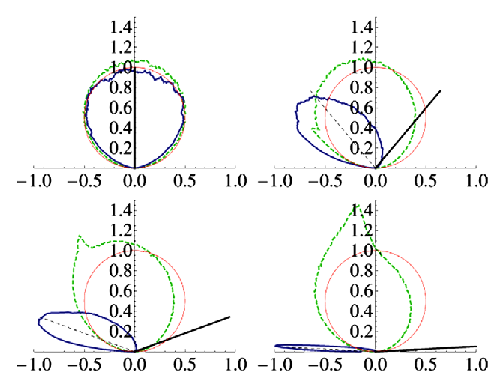
\includegraphics[width=6cm]{images/2.eps}
    \caption{This is a demo figure}
    \label{fig:demo1}
\end{figure}

\subsection{Вторичное распыление}

$IonShaper^{®}$ предпологает что переосаждённые атомы не распыляются и что отражённые ионы распыляются с таким же выходом как и падающие ионы. Чтобы посчитать достоверность этого предположения мы подсчитали средний выход распыления распылённых и обратно рассеянных ионов для нормального наклона ($Y_{ss}$ и $Y_{sb}$ соответственно) беря во внимание энергию распростронения распылённых ионов/обратно рассеяных ионов определённых симуляцией бинарных столкновений. Зависимость энергии нормально падающих распылённых ионов определенно с помощью аналитичной формулы. Т.к. в случае $Y_{ss}$ мы заинтересованы только в грубой оценке, мы приближаем выход распылённых $Si$ атомов распылением $Ar$ ионов.
Рис.3 показывает выход вторичного распыления $Y_{ss}$ и $Y_{sb}$. Для сильно наклонённыех наклон $Y_{sb}$ близок к распылённию падающих ионов
($Y_{s} = 1.47$),
но оно уменьшается значительно когда угол падения уменьшается (пример на 30\% в 80; угол боковой стенки на Рис. 1 между 77 и 86). Для контраста, средний выход распыления $Y_{ss}$ распылённых атомов скорее меньше и наверное незначительен в большенстве случаев.


\begin{figure}[h]
    \centering
    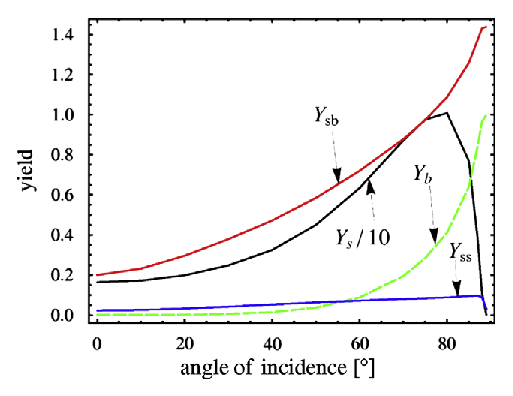
\includegraphics[width=6cm]{images/3.eps}
    \caption{This is a demo figure}
    \label{fig:demo1}
\end{figure}

\subsection{Не локальные эффекты}

Чтобы исследовать нелокальные эффекты мы взяли контур на рис.1 в 4.67с и посчитали основной поток распылённия в соответствии с разными моделями. Результаты полученные с локальной моделью показанны штрих-пунктирной линией на рис. 4, а результаты бинарного столкновения показанны сплошной линией. Можно заметить несколько удивительных отличий. Между 20нм и 50нм по абсциссе локальные результаты переоценивают поток. В первом случае это потому что луч ограничен \textgreater 20нм и вклад каскад отскоков столкновений ионов \textless 20нм пропущенно в результатах бинарного столкновия когда по иронии взято во внимание в локальной модели. В 50нм есть входящий поток \textgreater 50нм, но точки падений глубже чем если контур был бы расширен \textgreater 50нм с наклоном в \textless 50нм. Поэтому сложнее порождать отскоки от ионов в \textgreater 50нм чтобы вернуться к поверхности в \textless 50нм. Это отраженно в результатах бинарных столкновений но только в локальной модели. В 30нм видно два четких пика в локальной модели (положительный пик). Эти изминения в наклоне настолько стремительны что они не отраженны в результатах бинарных столкновений из-за эффекта размытия конечного размера каскадов отскоков.


\begin{figure}[h]
    \centering
    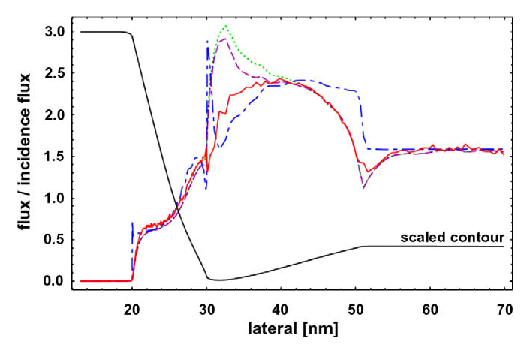
\includegraphics[width=6cm]{images/4.eps}
    \caption{This is a demo figure}
    \label{fig:demo1}
\end{figure}


Штриховая линия соответствует $IonShaper^{®}$ результатам полученным с табличной моделью отскоков описанных вместе с осаждённой моделью. Так же можно заметить что они совпадают с результатами бинарных столкновений в большей части случаев. Пик не представленный в результате бинарных столкновений может быть замечен только на дне микроямы (\textgreater 30нм). Это из-за того что путь от точки падения ион к точке назначения частично блокирован выгнутой поверхностю. Улучшенная модель описанная в конце секции 2.1 уменьшает этот пик, хотя некоторые отклонения от результатов бинарных столкновений остаются.

Наконец, рис. 5 показывает $IonShaper^{®}$ результаты вынужденного ионно-лучевого результата осаждения в 25нм границей 10К эВ $Ar$ лучём. Штриховая линия соответствует локальной модели когда сплошная линия представляет не локальную модель включая изменения отсков. Так же нужно заметить что конечные размеры каскада отскоков значительно увеличивают ширину осаждённгого столба. Этот эффект в основном выражен поскольку сравнительно низкая плотность отскоков вызывает значительный рост материала в ионно-лучевом осаждении.

\begin{figure}[h]
    \centering
    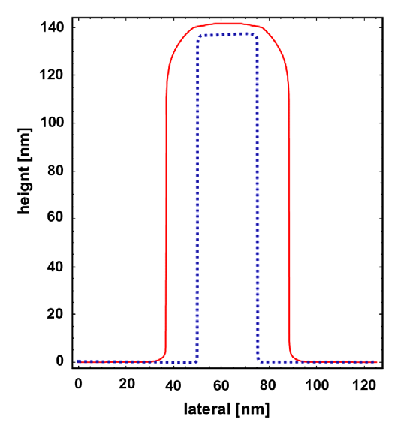
\includegraphics[width=6cm]{images/5.eps}
    \caption{This is a demo figure}
    \label{fig:demo1}
\end{figure}

\section{Выводы}
Наша оценка модели использованна для топографической симуляции ионой-лучевых процессов для 10К эВ $Ar$ ионов и $Si$ целей позволяет нам заключить следующее:

\begin{enumerate}
  \item Закон косинуса это только грубая аппроксимация углового распределения распылённых атомов. В особенности, распыление глубоких ям требует точного описания распределения на больщих обратных углах. Так же, зеркальное отражение это только грубая апроксимация для отражённых ионов. В обоих случаях реализация таблиц в топографическом симуляторе должна быть достачно хорошей.
  \item Как было показынно на рис. 1 распыление отражённых ионов может быть важным эффектом. Распыление распылённых частиц похоже несущественно из-за не значительного средней энергии распылённых атомов.
  \item Локальная модель распыления реализованная во всех топографических симуляторах на сегодня оказываеться достаточно неточна. Была предложенна модель основаная на пространственном распределении атомов на плоской поверхности и ожидается что она улучшает результаты на структурах малого размера. Нелокальная модель даже более важна для ионно-лучевого осаждения.
\end{enumerate}

Мы планируем расширить эту работу на другие энергии и типы ионов, изучать влияние предложенных моделей на форму поверхностей.

\section{Благодарности}

Эта работа было частично поддерженна Европейской коммисией путём финансирования проекта CHARPAN и Австрийским агенством продвижения, Австрийской нано инновационной программой, проектом NILaustria.

\end{document}
